\documentclass[../Matt_Gebert_Honours_Thesis.tex]{subfiles}
\begin{document}
	
%	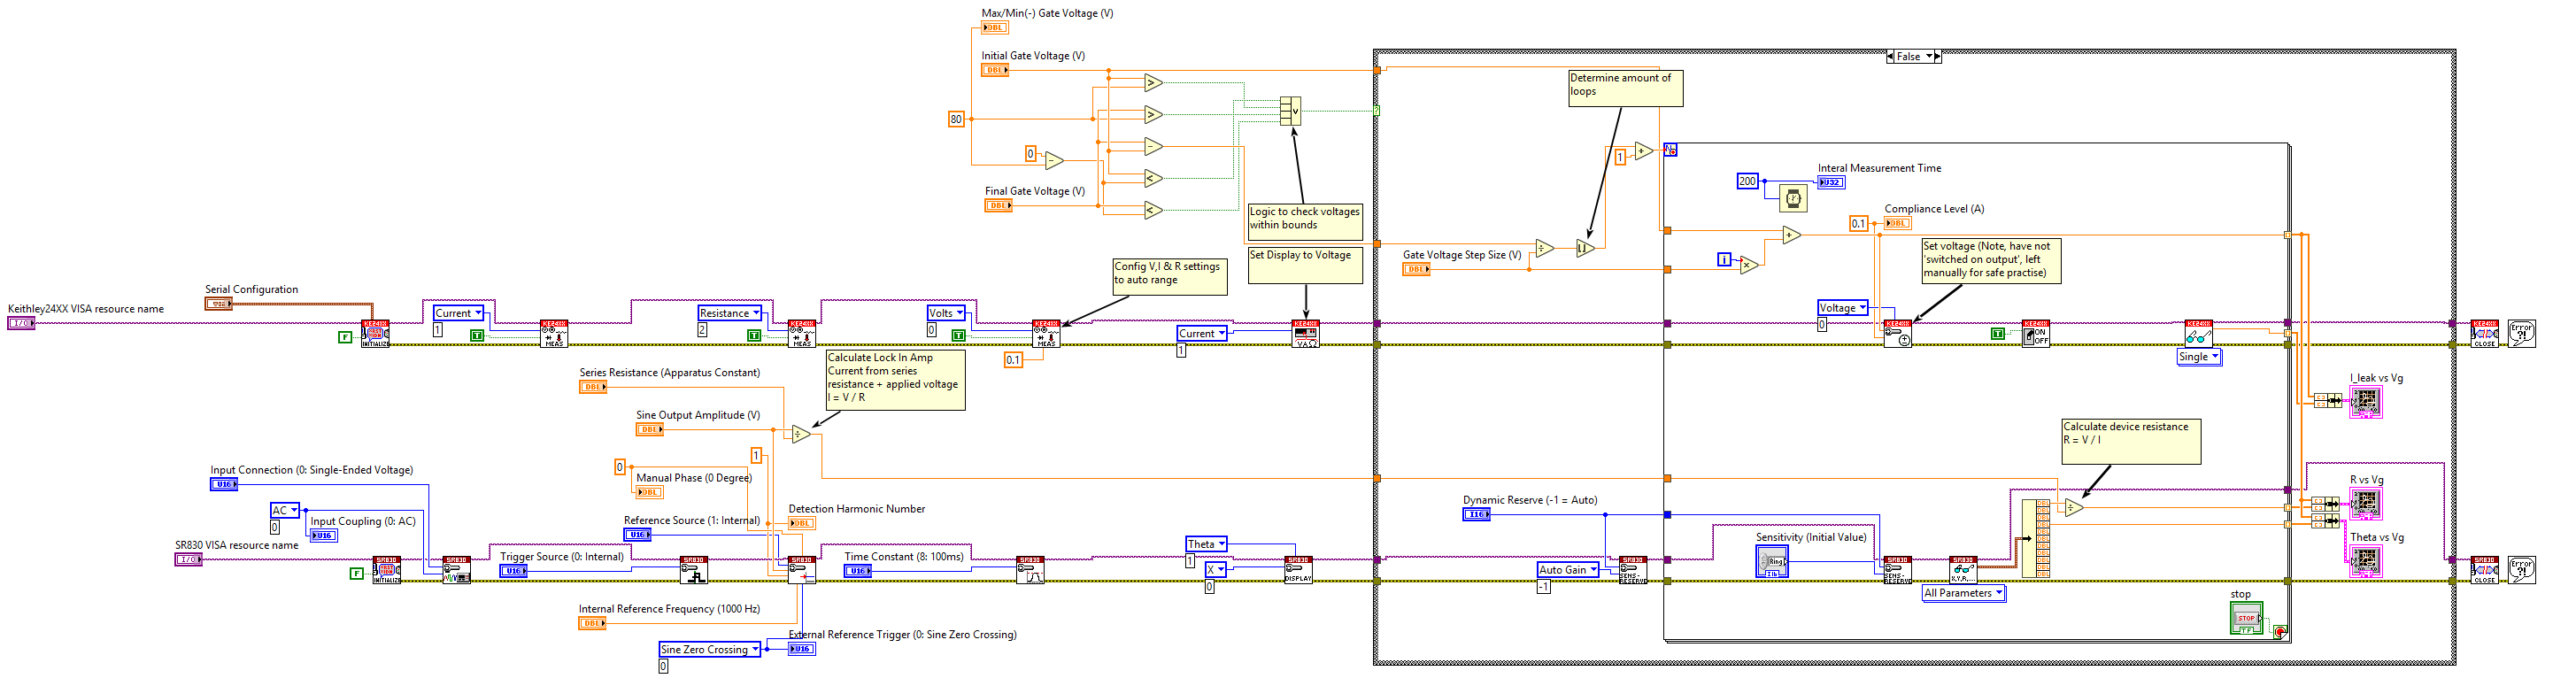
\includegraphics[width=\textwidth]{001_labview.png}
%	In \cref{chap:introduction}, I will outline what I hope to achieve in this project. I begin by discussing the theoretical properties of graphene and why it has attracted so much interest as an electronic material. I will also describe some challenges facing new computing technologies, including the use of dielectrics, and how my work contributes to realising solutions to new generations of this technology. I will outline a theoretical and experimental summary of the results to date seen in introducing dielectrics to graphene.

	\section{Preface}
	
	The mechanical exfoliation of atomically thin materials in 2004 sparked a flurry of research into many materials with unique properties. Graphene, the first of these, rose to prominence in research and has begun finding applications in industrial contexts. 
	
	Materials that are two dimensional restrict the movement of electrons to a plane. Becuase of this, these materials exhibit unique electronic properties. A clear example of this is a hexagonal lattice of carbon atoms, or graphene, which gives rise to a 'dirac' point in the band structure (see \cref{sec:electronic_dispersion}).
	
	\section{Transistors - the field effect}\label{sec:fet}
	\subsection{Conductivity in FETs}\label{sec:fet_cond}
	
	\subsection{Mobility in FETs}\label{sec:fet_mobil}
	
	\section{Graphene}\label{sec:graphene}
	\subsection{Electronic properties}\label{sec:electronic_properties}
	Why is it a good conductor?
	\subsubsection{Hybridisation}\label{sec:hybridisation}
	\subsubsection{Electronic dispersion}\label{sec:electronic_dispersion}
	\subsubsection{Charged puddling}\label{sec:charged_puddling}
	
	\section{Transport and scattering in graphene}\label{sec:transport&scattering}
	\subsection{Charged impurities}\label{sec:charged_impurities}
	\subsection{Phonon scattering}\label{sec:phonon_scattering}
	\subsection{Dielectric screening}\label{sec:dielectric_screening}
	\subsubsection{Charge screening}\label{sec:charge_screening}
	\subsubsection{Fine structure constant}\label{sec:fine_structure}
	\subsubsection{Tuning the fine structure constant}\label{sec:fine_structure_tuning}
	\subsubsection{High $\kappa$ materials}\label{sec:high_dielectrics}
	\subsection{Remote phonon scattering}\label{sec:remote_phonon_scattering}
	
	\section{}
	
	
	
\end{document}